% This is the Reed College LaTeX thesis template. Most of the work
% for the document class was done by Sam Noble (SN), as well as this
% template. Later comments etc. by Ben Salzberg (BTS). Additional
% restructuring and APA support by Jess Youngberg (JY).
% Your comments and suggestions are more than welcome; please email
% them to cus@reed.edu
%
% See https://www.reed.edu/cis/help/LaTeX/index.html for help. There are a
% great bunch of help pages there, with notes on
% getting started, bibtex, etc. Go there and read it if you're not
% already familiar with LaTeX.
%
% Any line that starts with a percent symbol is a comment.
% They won't show up in the document, and are useful for notes
% to yourself and explaining commands.
% Commenting also removes a line from the document;
% very handy for troubleshooting problems. -BTS

% As far as I know, this follows the requirements laid out in
% the 2002-2003 Senior Handbook. Ask a librarian to check the
% document before binding. -SN

%%
%% Preamble
%%
% \documentclass{<something>} must begin each LaTeX document
\documentclass[12pt,oneside]{reedthesis}
% Packages are extensions to the basic LaTeX functions. Whatever you
% want to typeset, there is probably a package out there for it.
% Chemistry (chemtex), screenplays, you name it.
% Check out CTAN to see: https://www.ctan.org/
%%
\usepackage{graphicx,latexsym}
\usepackage{amsmath}
\usepackage{amssymb,amsthm}
\usepackage{longtable,booktabs,setspace}
\usepackage{chemarr} %% Useful for one reaction arrow, useless if you're not a chem major
\usepackage[hyphens]{url}
% Added by CII
\usepackage{hyperref}
\usepackage{lmodern}
\usepackage{float}
\floatplacement{figure}{H}
% Thanks, @Xyv
\usepackage{calc}
% End of CII addition
\usepackage{rotating}

% Next line commented out by CII
%%% \usepackage{natbib}
% Comment out the natbib line above and uncomment the following two lines to use the new
% biblatex-chicago style, for Chicago A. Also make some changes at the end where the
% bibliography is included.
%\usepackage{biblatex-chicago}
%\bibliography{thesis}


% Added by CII (Thanks, Hadley!)
% Use ref for internal links
\renewcommand{\hyperref}[2][???]{\autoref{#1}}
\def\chapterautorefname{Chapter}
\def\sectionautorefname{Section}
\def\subsectionautorefname{Subsection}
% End of CII addition

% Added by CII
\usepackage{caption}
\captionsetup{width=5in}
% End of CII addition

% \usepackage{times} % other fonts are available like times, bookman, charter, palatino

% Syntax highlighting #22
  \usepackage{color}
  \usepackage{fancyvrb}
  \newcommand{\VerbBar}{|}
  \newcommand{\VERB}{\Verb[commandchars=\\\{\}]}
  \DefineVerbatimEnvironment{Highlighting}{Verbatim}{commandchars=\\\{\}}
  % Add ',fontsize=\small' for more characters per line
  \usepackage{framed}
  \definecolor{shadecolor}{RGB}{248,248,248}
  \newenvironment{Shaded}{\begin{snugshade}}{\end{snugshade}}
  \newcommand{\AlertTok}[1]{\textcolor[rgb]{0.94,0.16,0.16}{#1}}
  \newcommand{\AnnotationTok}[1]{\textcolor[rgb]{0.56,0.35,0.01}{\textbf{\textit{#1}}}}
  \newcommand{\AttributeTok}[1]{\textcolor[rgb]{0.77,0.63,0.00}{#1}}
  \newcommand{\BaseNTok}[1]{\textcolor[rgb]{0.00,0.00,0.81}{#1}}
  \newcommand{\BuiltInTok}[1]{#1}
  \newcommand{\CharTok}[1]{\textcolor[rgb]{0.31,0.60,0.02}{#1}}
  \newcommand{\CommentTok}[1]{\textcolor[rgb]{0.56,0.35,0.01}{\textit{#1}}}
  \newcommand{\CommentVarTok}[1]{\textcolor[rgb]{0.56,0.35,0.01}{\textbf{\textit{#1}}}}
  \newcommand{\ConstantTok}[1]{\textcolor[rgb]{0.00,0.00,0.00}{#1}}
  \newcommand{\ControlFlowTok}[1]{\textcolor[rgb]{0.13,0.29,0.53}{\textbf{#1}}}
  \newcommand{\DataTypeTok}[1]{\textcolor[rgb]{0.13,0.29,0.53}{#1}}
  \newcommand{\DecValTok}[1]{\textcolor[rgb]{0.00,0.00,0.81}{#1}}
  \newcommand{\DocumentationTok}[1]{\textcolor[rgb]{0.56,0.35,0.01}{\textbf{\textit{#1}}}}
  \newcommand{\ErrorTok}[1]{\textcolor[rgb]{0.64,0.00,0.00}{\textbf{#1}}}
  \newcommand{\ExtensionTok}[1]{#1}
  \newcommand{\FloatTok}[1]{\textcolor[rgb]{0.00,0.00,0.81}{#1}}
  \newcommand{\FunctionTok}[1]{\textcolor[rgb]{0.00,0.00,0.00}{#1}}
  \newcommand{\ImportTok}[1]{#1}
  \newcommand{\InformationTok}[1]{\textcolor[rgb]{0.56,0.35,0.01}{\textbf{\textit{#1}}}}
  \newcommand{\KeywordTok}[1]{\textcolor[rgb]{0.13,0.29,0.53}{\textbf{#1}}}
  \newcommand{\NormalTok}[1]{#1}
  \newcommand{\OperatorTok}[1]{\textcolor[rgb]{0.81,0.36,0.00}{\textbf{#1}}}
  \newcommand{\OtherTok}[1]{\textcolor[rgb]{0.56,0.35,0.01}{#1}}
  \newcommand{\PreprocessorTok}[1]{\textcolor[rgb]{0.56,0.35,0.01}{\textit{#1}}}
  \newcommand{\RegionMarkerTok}[1]{#1}
  \newcommand{\SpecialCharTok}[1]{\textcolor[rgb]{0.00,0.00,0.00}{#1}}
  \newcommand{\SpecialStringTok}[1]{\textcolor[rgb]{0.31,0.60,0.02}{#1}}
  \newcommand{\StringTok}[1]{\textcolor[rgb]{0.31,0.60,0.02}{#1}}
  \newcommand{\VariableTok}[1]{\textcolor[rgb]{0.00,0.00,0.00}{#1}}
  \newcommand{\VerbatimStringTok}[1]{\textcolor[rgb]{0.31,0.60,0.02}{#1}}
  \newcommand{\WarningTok}[1]{\textcolor[rgb]{0.56,0.35,0.01}{\textbf{\textit{#1}}}}

% To pass between YAML and LaTeX the dollar signs are added by CII
\title{Spatiotemporal modeling and predicting of average flows in Scotland based on generalized additive models}
\author{Mengran Li}
% The month and year that you submit your FINAL draft TO THE LIBRARY (May or December)
\date{December 2021}
\division{Mathematics and Natural Sciences}
\advisor{Advisor F. Name}
\institution{University of Glasgow}
\degree{Master of Science}
%If you have two advisors for some reason, you can use the following
% Uncommented out by CII
% End of CII addition

%%% Remember to use the correct department!
\department{School of Mathematics and Statistics}
% if you're writing a thesis in an interdisciplinary major,
% uncomment the line below and change the text as appropriate.
% check the Senior Handbook if unsure.
%\thedivisionof{The Established Interdisciplinary Committee for}
% if you want the approval page to say "Approved for the Committee",
% uncomment the next line
%\approvedforthe{Committee}

% Added by CII
%%% Copied from knitr
%% maxwidth is the original width if it's less than linewidth
%% otherwise use linewidth (to make sure the graphics do not exceed the margin)
\makeatletter
\def\maxwidth{ %
  \ifdim\Gin@nat@width>\linewidth
    \linewidth
  \else
    \Gin@nat@width
  \fi
}
\makeatother

% From {rticles}
\newlength{\csllabelwidth}
\setlength{\csllabelwidth}{3em}
\newlength{\cslhangindent}
\setlength{\cslhangindent}{1.5em}
% for Pandoc 2.8 to 2.10.1
\newenvironment{cslreferences}%
  {}%
  {\par}
% For Pandoc 2.11+
% As noted by @mirh [2] is needed instead of [3] for 2.12
\newenvironment{CSLReferences}[2] % #1 hanging-ident, #2 entry spacing
 {% don't indent paragraphs
  \setlength{\parindent}{0pt}
  % turn on hanging indent if param 1 is 1
  \ifodd #1 \everypar{\setlength{\hangindent}{\cslhangindent}}\ignorespaces\fi
  % set entry spacing
  \ifnum #2 > 0
  \setlength{\parskip}{#2\baselineskip}
  \fi
 }%
 {}
\usepackage{calc} % for calculating minipage widths
\newcommand{\CSLBlock}[1]{#1\hfill\break}
\newcommand{\CSLLeftMargin}[1]{\parbox[t]{\csllabelwidth}{#1}}
\newcommand{\CSLRightInline}[1]{\parbox[t]{\linewidth - \csllabelwidth}{#1}}
\newcommand{\CSLIndent}[1]{\hspace{\cslhangindent}#1}

\renewcommand{\contentsname}{Table of Contents}
% End of CII addition

\setlength{\parskip}{0pt}

% Added by CII

\providecommand{\tightlist}{%
  \setlength{\itemsep}{0pt}\setlength{\parskip}{0pt}}

\Acknowledgements{
First and foremost, I would like to thank the team of supervisors at the School of Statistics, University of Glasgow, who provided excellent advice and supervision for my project. I thank them for their profound knowledge, patience and enthusiasm.

Secondly, I would like to express my gratitude to all the teachers in the School of Statistics at the University of Glasgow for leading me to explore the vast world of statistics. In particular, Dr.~Daniela Castro-Camilo has inspired me with her wisdom and passion for statistics. I have benefited deeply from our discussions on statistics.

I am especially grateful to my parents, who always give me unconditional support and are always my strongest backup. Their respect and understanding empower me to pursue my dreams. Sincere thanks to my friends who give me so much encouragement and give me a sense of warmth. To Zuqi Shen, for growing up together and motivating each other.

To my life partner: Zhang Yue. Thank you for bringing me to experience love. Thank you for your bravery, sweetness and tenderness. Thank you for writing love in the period of Cholera with me. For you, thousands of times over.
}

\Dedication{

}

\Preface{

}

\Abstract{
Global climate change affects flows, which is crucial for policymaking in agriculture, hydropower generation, and conservation of natural habitats. The aim of this paper is to discover the spatial and temporal characteristics of flows in Scotland and to develop effective predictive models. Based on data from 65 stations between 1989 to 2015, this paper develops generalised additive models (GAMs) with temporal, seasonal, and spatial as explanatory variables and catchment area and maximum elevation as covariates, and selects the best model through AIC and BIC criteria, tests significance through hypothesis testing, and tests the effectiveness of prediction by k-fold cross-validation. The results reveal that Scottish flows show a clear upward trend and a seasonal effect of smaller summer flows and larger winter flows. Spatially flows are smaller at higher altitudes than at lower ones, and flows are less on the west coast than on the east coast. The study predicts a continued increase in average flows in Scotland from 2021 to 2030.
}

	\usepackage{setspace}\onehalfspacing
	\usepackage{booktabs}
 \usepackage{longtable}
 \usepackage{array}
 \usepackage{multirow}
 \usepackage{wrapfig}
 \usepackage{float}
 \usepackage{colortbl}
 \usepackage{pdflscape}
 \usepackage{tabu}
 \usepackage{threeparttable}
 \usepackage{threeparttablex}
 \usepackage[normalem]{ulem}
 \usepackage{makecell}
 \usepackage{xcolor}
% End of CII addition
%%
%% End Preamble
%%
%
\begin{document}

% Everything below added by CII
  \maketitle

\frontmatter % this stuff will be roman-numbered
\pagestyle{empty} % this removes page numbers from the frontmatter
  \begin{acknowledgements}
    First and foremost, I would like to thank the team of supervisors at the School of Statistics, University of Glasgow, who provided excellent advice and supervision for my project. I thank them for their profound knowledge, patience and enthusiasm.

    Secondly, I would like to express my gratitude to all the teachers in the School of Statistics at the University of Glasgow for leading me to explore the vast world of statistics. In particular, Dr.~Daniela Castro-Camilo has inspired me with her wisdom and passion for statistics. I have benefited deeply from our discussions on statistics.

    I am especially grateful to my parents, who always give me unconditional support and are always my strongest backup. Their respect and understanding empower me to pursue my dreams. Sincere thanks to my friends who give me so much encouragement and give me a sense of warmth. To Zuqi Shen, for growing up together and motivating each other.

    To my life partner: Zhang Yue. Thank you for bringing me to experience love. Thank you for your bravery, sweetness and tenderness. Thank you for writing love in the period of Cholera with me. For you, thousands of times over.
  \end{acknowledgements}

  \hypersetup{linkcolor=black}
  \setcounter{secnumdepth}{2}
  \setcounter{tocdepth}{2}
  \tableofcontents

  \listoftables

  \listoffigures
  \begin{abstract}
    Global climate change affects flows, which is crucial for policymaking in agriculture, hydropower generation, and conservation of natural habitats. The aim of this paper is to discover the spatial and temporal characteristics of flows in Scotland and to develop effective predictive models. Based on data from 65 stations between 1989 to 2015, this paper develops generalised additive models (GAMs) with temporal, seasonal, and spatial as explanatory variables and catchment area and maximum elevation as covariates, and selects the best model through AIC and BIC criteria, tests significance through hypothesis testing, and tests the effectiveness of prediction by k-fold cross-validation. The results reveal that Scottish flows show a clear upward trend and a seasonal effect of smaller summer flows and larger winter flows. Spatially flows are smaller at higher altitudes than at lower ones, and flows are less on the west coast than on the east coast. The study predicts a continued increase in average flows in Scotland from 2021 to 2030.
  \end{abstract}

\mainmatter % here the regular arabic numbering starts
\pagestyle{fancyplain} % turns page numbering back on

\hypertarget{intro}{%
\chapter{Introduction}\label{intro}}

\hypertarget{background}{%
\section{Background}\label{background}}

The UK hosted the 26th United Nations Conference of the Parties on Climate Change (COP26) in Glasgow from 31 October to 13 November 2021, uniting the world in the fight against climate change. Human activities have led to increased CO2 emissions and global warming with a range of impacts, which has already caused widespread concern (Naveau, Hannart, \& Ribes, 2020). Climate change poses challenges for the management of water resources, particularly in the catchment area (Griffiths et al., 2006). Hydrological forecasting is highly profitable for decisions on hydropower, agriculture and, conservation of natural habitats (Harrigan, Prudhomme, Parry, Smith, \& Tanguy, 2018).

In the field of hydrology, physical models based on hydrological processes are still perceived to be the best models for streamflow prediction, but data-driven approaches have also flourished in recent years, with machine learning in particular being widely used (Iorgulescu \& Beven, 2004). Methods such as artificial neural networks (ANN), regression trees and, support vector machines are proved to offer strong predictive capabilities (Solomatine \& Ostfeld, 2008). Nevertheless, these methods usually suffer from over-fitting problems and are difficult to explain. The generalized additive models (GAMs) can also accurately predict complex temporal-spatial distributions and compared to methods such as ANN, they offer the advantages of better interpretability, visualization and, the availability of formal statistical hypothesis tests (Shortridge, Guikema, \& Zaitchik, 2016). It makes the application of GAMs for the interpretation and prediction of hydrological data an attractive option.

\hypertarget{aims-of-the-proposed-research}{%
\section{Aims of the proposed research}\label{aims-of-the-proposed-research}}

A series of studies have shown that since the 1960s Scotland has had a wetter (especially in the west) and warmer climate on average (A. R. Black, 1995; Soulsby, Black, \& Werritty, 2002; Werritty \& Sugden, 2012). This trend is expected to continue throughout the 21st century (Werritty \& Sugden, 2012). However, the hydrology of Scotland is still insufficiently studied. Only (Franco-Villoria, Scott, \& Hoey, 2018) has conducted a complete research on Scottish flows, except for a complete study by Andrew R. Black \& Werritty (1997). Most of the current literature has investigated only single or several gauging stations instead of flows across Scotland (Prosdocimi, Kjeldsen, \& Svensson, 2014). Therefore, the aim of this research is to explore a panoramic view of Scottish flows for long-term based on a large dataset and to propose a flexible framework of effective prediction based on the GAM.

\hypertarget{questions-of-interest}{%
\section{Questions of interest}\label{questions-of-interest}}

In order to achieve the above objectives, three specific research questions need to be addressed.
\begin{enumerate}
\def\labelenumi{\arabic{enumi}.}
\item
  How the average daily flows in Scotland vary over time?
\item
  What are the spatial patterns of the average daily flows in Scotland?
\item
  Are there covariates that contribute substantially to the forecast of Scottish flows?
\end{enumerate}
Chapter 2 introduces the geographical features of Scotland and summarises the data set utilised in this paper. Chapter 3 constructs the methodology for modelling discharge data and the results are reported and discussed in Chapter 4. Chapter5 concludes and discusses the results and limitations of this study.

\hypertarget{math-sci}{%
\chapter{Region of study and data}\label{math-sci}}

\hypertarget{scottish-climatic-and-geography-features}{%
\section{Scottish climatic and geography features}\label{scottish-climatic-and-geography-features}}

Scotland is located in Western Europe, the northern part of the British Isle and the Atlantic Ocean in the West. It has a temperate marine climate. The four seasons in Scotland are winter (December to February), spring (March to May), summer (June to August), and autumn (September to November).
Overall Scotland is rainy all year round but varies vastly from region to region. Research evidence shows that the dry season is from the 1960s to the 1970s, and the rainy season is from the late 1980s to the early 1990s (A. R. Black, 1995; Smith \& Bennett, 1994).

Fig. \ref{fig:geo} presents a geographical map of Scotland, drawn with the R package leaflet, modified from the world map provided by ESRI. There are three main geographical divisions in Scotland, the Highlands and Islands in the northwest, the Central Lowlands and Southern Uplands. The average altitude in the northwest exceeds 1300m, blocking the westerly flow from the Atlantic Ocean, where there is abundant precipitation. On the east coast, the terrain is relatively flat, suitable for animal husbandry and farming (Soulsby, Black, \& Werritty, 2002). The Grampian Mountains in the south of the Highlands are the highest on the British island, and the highest peak Ben Nevis reaches 1343m. The central lowland is a rift valley that spans the narrow waist of Scotland from the head of the Firth of Clyde in the west to the Firth of Forth in the east. These fjords provide a valuable way to the sea. The flat terrain here is the main agricultural area in Scotland. The influence of geology on hydrology lead to more subdued hydrological regimes here (Soulsby, Black, \& Werritty, 2002). The southern highlands are usually no more than 600 meters above sea level. The southern highlands usually have an altitude of no more than 600, and snow accounts for 30\% of the average annual precipitation. The complex topography and diverse climate pose considerable challenges to the modelling and prediction of Scottish flows.
\begin{figure}

{\centering \includegraphics[width=0.7\linewidth]{files/map} 

}

\caption{\label{fig:geo} Geographical map of Scotland, modified from the world map provided by ESRI.}\label{fig:unnamed-chunk-4}
\end{figure}
\hypertarget{study-catchments-and-datasets}{%
\section{Study catchments and datasets}\label{study-catchments-and-datasets}}

Our analysis of stream flows is based on data recorded in Scotland, made available by the Scottish Environment Protection Agency (SEPA) and the National River Flow Archive(NRFA). The data set contains observations from 65 gauging stations along different rivers. The streamflow over a region, which is called as catchment, is drained to the gauging station. The catchment boundary in UK is divided within 50\(m\) grid by the Centre for Ecology \& Hydrology's Integrated Hydrological Digital Terrain Model (IHDTM, Kral, 2015). Fig. \ref{fig:map} displays the locations of gauging stations on a map. The observation period spans 27 years for all stations from January 1, 1989, to December 31, 2015. This dataset has no missing values.
\begin{figure}
\centering
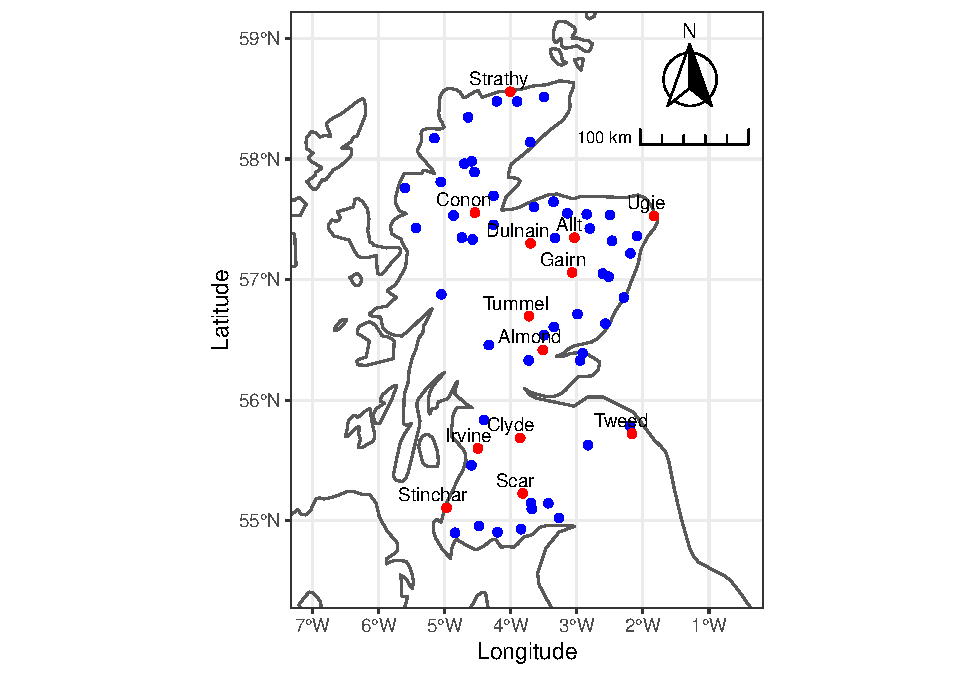
\includegraphics{thesis_files/figure-latex/unnamed-chunk-5-1.pdf}
\caption{\label{fig:unnamed-chunk-5}\label{fig:map} Locations of 65 gauging stations. Red dots are the locations of selected gauging stations for initial exploration.}
\end{figure}
Due to the computational cost of large datasets, we chose a subset of 10\% of the observations for the initial analysis and eventually applied the final model to the full data. The method is introduced in detail in Chapter 3. The red dots are the selected gauging stations in Fig. \ref{fig:map} and we can note that they are distributed throughout the Scottish region.

\hypertarget{variables-of-interest}{%
\section{Variables of interest}\label{variables-of-interest}}

Inside the dataset, we exact six variables, Flow, Catchment Area, Max Altitude, Year, doy, and bivariate variable coordinates (Longitude, Altitude) to analyse the flow change.

Flow (\(m^3/s\)) is the daily average flow in each gauge station. It is regarded as the response variable in the research of Scottish average flow. The range of flow in Scotland is from 0.001 \(m^3/s\) to 1349 \(m^3/s\) with the mean 18.7181\(\pm\) 41.0709 \(m^3/s\).
\begin{table}[!h]

\caption{\label{tab:unnamed-chunk-6}\label{tab:summary} Summary statistics on daily flow, catchment area and maximum altitude in the catchment.}
\centering
\fontsize{10}{12}\selectfont
\begin{tabular}[t]{lrrrrrrr}
\toprule
Variable & Mean & SD & Min. & 1st Q. & Median & 3rd Q. & Max.\\
\midrule
Flow & 18.7181 & 41.0709 & 0.001 & 1.934 & 5.285 & 17.29 & 1349.0\\
Catchment.Area & 556.6354 & 767.1688 & 60.000 & 171.000 & 239.000 & 551.40 & 4390.0\\
Max.Altitude & 784.5708 & 282.5950 & 233.700 & 568.700 & 803.100 & 1007.30 & 1308.9\\
\bottomrule
\end{tabular}
\end{table}
Flow shows an obvious positive skew distribution.

Table \ref{tab:summary} are summary statistics of flow data, catchment area, and maximum altitude in the catchment. Fig. \ref{fig:relation} shows the relationship between river flow and other variables of interest.

The surface area of the region projected onto a horizontal plane is defined as Catchment Area (\(km^2\)). In our dataset, the largest catchment has an area of 4390 \(km^2\) and the smallest one is only 60 \(km^2\). The mean area of all catchments is 556.64 \(\pm\) 767.17 \(km^2\). The distribution of the catchment area is positively skewed. Fig. \ref{fig:relation}(a) displays the potential positive relationship between Catchment Area and average flow. The y-axis is the mean flow at a gauging station for the entire observing period and the x-axis is the responding catchment area. The blue line is the coefficient fitted by simple linear regression. The Max Altitude (\(m\)) is the maximum altitude inside a catchment. It ranges from 233.7 \(m\) to 1308.9 \(m\) with mean 784.57 \(\pm\) 282.59 \(m\). Fig. \ref{fig:relation}(b) shows that the catchments with the larger area have higher average flow.

The temporal effect is represented by the Year (1989-2015). Fig. \ref{fig:relation}(c) indicates that the annual mean flow fluctuates stationary. The variable doy is the day of the year, for example, 1st January is the first day of a year, thus the doy is 1 and 31st December is the last day of a year, therefore the doy is 365. We remove the data on 29th Feb to ensure that the doy is the same every year. The deleted observations are close to the values nearly so that the treatment does not influence our results. Thus N = 65 × 27 × 365 = 640575, that is, 27 years of 365 daily observations in each station. Because the flow trend of the month is similar to the doy (1-365), we choose the doy to detect the seasonal pattern. Fig \ref{fig:relation}(d) reveals a trend that the average flow decreases to the middle of the year and then increases, say, the flow goes up in winter and falls down in summer.
\begin{figure}
\centering
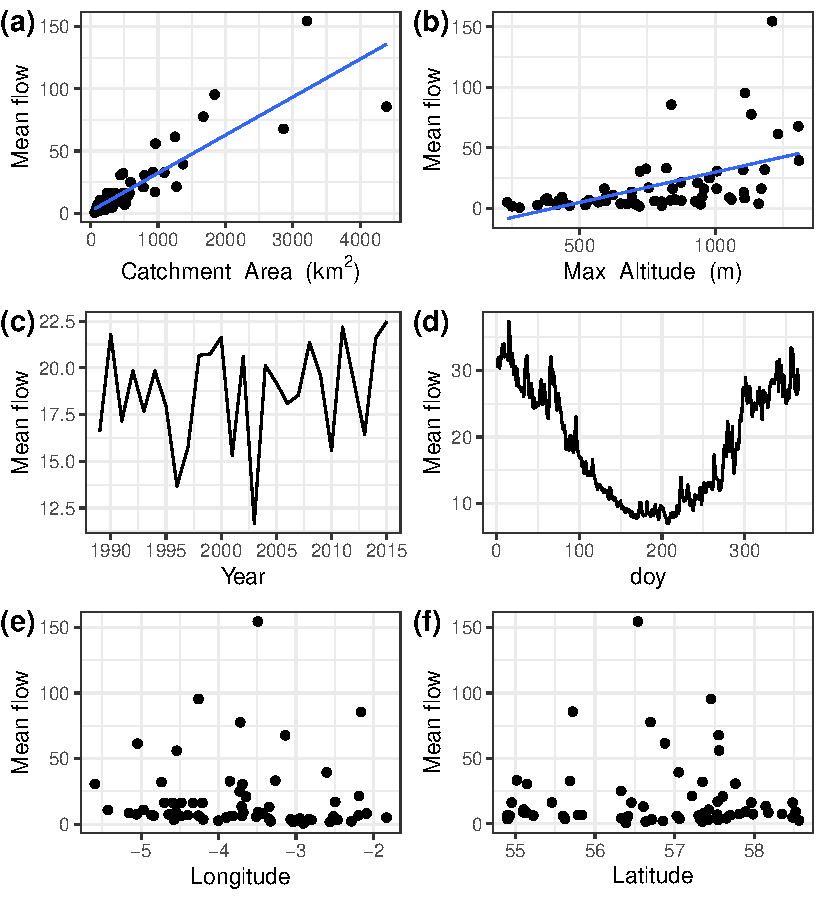
\includegraphics{thesis_files/figure-latex/unnamed-chunk-7-1.pdf}
\caption{\label{fig:unnamed-chunk-7}\label{fig:relation} Relationships of corvarites and flow.}
\end{figure}
We use coordinate to evaluate the spatial effect, which includes longitude and latitude, whose units are a degree. The distribution of gauging stations are from -5.60\(^\circ\)E to -1.83\(^\circ\)E and from 54.90\(^\circ\)N to 58.56\(^\circ\)N. The Fig \ref{fig:relation}(e) and Fig \ref{fig:relation}(f) are scatter plots of gauging station longitude and latitude vs average flow respectively. In longitude, the flow at the middle region is more likely to be large, and the same pattern is identified in latitude.

\hypertarget{ref-labels}{%
\chapter{Description of the methods}\label{ref-labels}}

\hypertarget{formulation-of-statistical-models}{%
\section{Formulation of statistical models}\label{formulation-of-statistical-models}}

One of the most well-known tools for assessing the pattern of flow data is the linear models, which are expressed as Eq. \ref{eq:lm}.
\begin{equation}
g(E(y_i))=\beta_0+\beta_1 x_{1i}+\beta_2 x_{2i} + \beta_3 t_i + \beta_4 d_i + \beta_5z_{1i}+\beta_6z_{2i}+\varepsilon_i,\;i=1,\dots,n, \label{eq:lm}
\end{equation}
where \(g(\cdot)\) is a known link function. We assume the flow data \(y_{i}\) follows the exponential family of distributions \(f(y_{i})=\exp\{\frac{y_{i}a_{i}-b(a_{i})}{\phi}+c(y_{i},\phi)\}\), \(\varepsilon_i\sim N(0,\sigma^2)\), where \(a_{i}\) is canonical parameter, \(b(\cdot)\) and \(c(\cdot)\) are known functions and \(\phi\) is the dispersion parameter. The variables \(x_1\) and \(x_2\) are catchment area and max altitude respectively, \(t_i\) and \(d_i\) denote time (year) and doy (day of the year), which represent time effect and seasonal effect respectively, and \(z_1\) and \(z_2\) represent spatial effect, say, longitude and latitude in coordinates.

Given the temporal and spatial complexity of river data, linear regression may not be appropriate in this research, so a flexible approach is employed. A spatiotemporal additive model (main effects model) of river flows can be expressed as Eq. \ref{eq:gammain}.
\begin{equation}
g(E(y_i)) =\beta_0+\beta_1 x_{1i}+\beta_2 x_{2i}+s_1(t_i) + s_2(d_i) + s_3(z_i)+\varepsilon_i,\;i=1,\dots,n, \label{eq:gammain}
\end{equation}
where \(s_1(t)\) and \(s_2(d)\) denote smooth functions for time (year) and doy (day of the year), and \(s_3(z)\) is a bivariate smooth function for coordinates (longitude, latitude). The previous two functions represent the time and seasonal effects respectively and the third function represents the spatial effects. The bivariate smooth function \(s_3(z)\) = \(s_3(Longitude, Latitude)\) is the tensor product of the marginal B-spline basis on the individual variables Longitude and Latitude.

Furthermore, we established a model with \(s_4(t_i,d_i)\), interaction effect of time and seasonal effects as Eq. \ref{eq:inter}
\begin{equation}
g(E(y_i)) =\beta_0+\beta_1 x_{1i}+\beta_2 x_{2i} +s_1(t_i) + s_2(d_i) + s_3(z_i)+s_4(t_i,d_i)+\varepsilon_i,\;i=1,\dots,n. \label{eq:inter}
\end{equation}
Finally, we proposed a full model with \(s_5(t_i,z_i)\) and \(s_6(d_i,z_i)\), which represent interaction effects of time-space and season-space respectively as Eq. \ref{eq:full}.
\begin{equation}
  \begin{array}{l}
g(E(y_i)) = \beta_0+\beta_1x_{1i}+\beta_2x_{2i} +s_1(t_i) + s_2(d_i) + s_3(z_i)\\+s_4(t_i,d_i)+s_5(t_i,z_i) +s_6(d_i,z_i)+ \varepsilon_i,\;i=1,\dots,n. \label{eq:full}
  \end{array}
\end{equation}
Because of the positive skewness of the flow data, we fitted the models using different family and link functions. The linear model is the base model to be compared and is defined as \(Model_{1\cdot}\). The models expressed by Eq.(\ref{eq:lm}, \ref{eq:gammain}, \ref{eq:inter}, \ref{eq:full}) are labelled as \(Model_{11}\), \(Model_{12}\), \(Model_{13}\) and \(Model_{14}\) correspondingly. The log-norm and Gamma are two common choices of data distributions in hydrology (Bobee, Perreault, \& Ashkar, 1993). We defined the models with norm distribution and log link function and models with gamma distribution and log link function as \(Model_{2\cdot}\) and \(Model_{3\cdot}\) respectively. The logarithmic transformation is also a normal treatment of positively skewed data in statistics, so we defined these models as \(Model_{4\cdot}\). All candidate models can be annotated as \(Model_{ij}\), where \(i=1,\dots,4\) represents which distribution the response is and \(j=1,\dots,4\) represents which formula the models with different variables belong to. The response distributions of the candidate models are listed in Table \ref{tab:model}.
\begin{table}[!h]

\caption{\label{tab:unnamed-chunk-8}\label{tab:model} Distribution family and link function of candidate models}
\centering
\fontsize{10}{12}\selectfont
\begin{tabular}[t]{llll}
\toprule
Model & Response & Family & Link function\\
\midrule
$Model_{1{\cdot}}$ & Flow & gaussion & identity\\
$Model_{2{\cdot}}$ & Flow & gaussion & log\\
$Model_{3{\cdot}}$ & Flow & gamma & log\\
$Model_{4{\cdot}}$ & log(Flow) & gaussion & indentity\\
\bottomrule
\end{tabular}
\end{table}
\hypertarget{model-fitting-selection-and-checks}{%
\section{Model fitting, selection and checks}\label{model-fitting-selection-and-checks}}

The computation of GAMs is painful due to the large dataset and plenty of parameters. We took the following means to decrease the model fitting cost.

Instead of the gam function in the mgcv package (Wood, Goude, \& Shaw, 2014), which is generally used to fit GAMs, bam function from the same package, provides an efficient tool to fit GAMs in the large data set. We apply the bam function to our data. For the univariate items, we choose cubic B-spline basis functions with the secondary penalty. For the bivariate items and interaction effect items, we employ the cubic regression splines, which are penalized by the conventional integrated square second derivative cubic spline penalty. The smoothness selection criteria is the fast restricted maximum likelihood (fREML) based on the restricted maximum likelihood REML criteria (Li \& Wood, 2019; Wood, Goude, \& Shaw, 2014; Wood, Li, Shaddick, \& Augustin, 2017) but much faster than which.

For each response distribution, the above models \(Model_{i\cdot}\) as Eq.(\ref{eq:lm}, \ref{eq:gammain}, \ref{eq:inter}, \ref{eq:full}) were fitted respectively. GAMs employ more parameters, which leads to a better fit, but is also complicated. The Akaike Information Criterion (AIC, Akaike, 1998), Bayesian information criterion (BIC, Buckland, Burnham, \& Augustin, 1997) are generally adopted for model selection. They strike a balance between the goodness of fit and freedom. The general likelihood ratio test (GLRT) and F-test are used to perform the significance tests for model comparison (Scheipl, Greven, \& Küchenhoff, 2008).

We took 20\% of the total 65 stations, i.e.~13 stations, for initial exploration and applied the appropriate model to the full dataset. Please see Appendix \ref{infor} for more information on the 13 gauging stations randomly selected. For each distribution \(Model_{i\cdot}\), the following procedure was executed. Four models \(Model_{ij},j=1,\dots,4\) were fitted separately and the candidate models were compared and the best model selected by AIC and BIC. The four models \(Model_{ij},j=1,\dots,4\) are nested, so the selected best model is tested for significance by GLRT and F-test and the best model is determined. Finally, the four selected models were compared by deviance explained rate (DER) to determine the final best model.

Once we have chosen the best model, we checked the residuals to dialogue whether we have built the model correctly. We identified whether there was spatial autocorrelation and temporal autocorrelation.

\hypertarget{predictive-performance}{%
\section{Predictive performance}\label{predictive-performance}}

Model selection is based on information criteria, however, it focuses on how well the model fits the observed data, meaning that the model may perform poorly in prediction. We used the cross validation method to assess the predictive efficiency of the models. Given the large size of our model, we chose the k-folder cross-validation method to obtain prediction quality. The k folder method is flexible for big datasets and provides more accurate results than the hold out method, although the value of k is limited (Yadav \& Shukla, 2016). When the number of instances is between 150,000 and 1,000,000, a value of 3-5 is recommended for k. Thus, we divide the entire dataset into 5 random subsets. This process is described as the following steps.
\begin{enumerate}
\def\labelenumi{\arabic{enumi}.}
\item
  The 65 stations were randomly divided into 5 groups, each group containing 13 stations. The complete dataset was divided into 5 subsets accordingly. We denote the 65 gauging stations as \(\pmb{z}_{rk},r=1,\dots,5,k=1,\dots,13\), where \(r=1\) is the index of the 5 groups and \(k\) is the index of the 13 gauging stations in each group.
\item
  A subset \(\pmb{u}_r=(u(\pmb{z}_{r_1}),\dots,u(\pmb{z}_{r13}))\) is picked as the test set and other four as the training set \(\pmb{u}_{-r}=(\pmb{u}_1,\dots,\pmb{u}_{r-1},\pmb{u}_{r+1},\dots,\pmb{u}_5)\), where \(u(\pmb{z}_{rk})\) is the observation from \(rk^{th}\) gauging station.
\item
  The model was fitted with the training set \(\pmb{u}_{-r}\) and the process was predicted on the test set \(\pmb{u}_{r}\) as \(\pmb{P}_{\pmb{u}_{-r}}\).
\end{enumerate}
In order to achieve a robust result, we used three different criteria to evaluate our models. Root mean square prediction error (RMSPE) is a popular statistical tool for error accuracy criteria in hydrology (Kisi \& Cimen, 2011), which is defined as

\[RMSPE=\sqrt{\frac{1}{n_r}\sum_{i=1}^{n_r}(\pmb{u}_{r}-P_{\pmb{u}_{-r}})^2},\] where \(n_r\) is the number of observations in the \(r^{th}\) group.

Mean absolute prediction error (MAPE) has also been used to compare different models in hydrology (Kisi \& Cimen, 2011), which is defined as

\[MAPE=\frac{1}{n_r}\sum_{i=1}^{n_r}|\pmb{u}_{r}-P_{\pmb{u}_{-r}}|.\]

Similarly, Median absolute prediction error (MdAPE Shcherbakov et al., 2013), is defined as

\[MdAPE=\underset {i=1,\dots,n} {median}|\pmb{u}_{r}-P_{\pmb{u}_{-r}}|.\]

After confirming the good ability in prediction, we fitted the select model into the full data and analysed how trends in flows varied over time and space.

\hypertarget{conclusion}{%
\chapter{Analysis of the data}\label{conclusion}}

\hypertarget{selected-best-model}{%
\section{Selected best model}\label{selected-best-model}}

We fitted the candidate models via the bam function in the mgcv package (Wood, Goude, \& Shaw, 2014) as appendix 1. All the smooth parameters were determined automatically by the fREML criterion. The 2nd derivative of penalty was imposed on the splines. For the choice of knots, We need a sufficiently large k as the basis dimension which can represent the smooth term with sufficient degrees of freedom. Nevertheless, there is no clear definition of how large k should be. We therefore chose k=6 for all items to keep the k as large as possible while ensuring that the computational cost is acceptable. We compared a total of 16 models as Table \ref{tab:result}.
\begin{table}[!h]

\caption{\label{tab:unnamed-chunk-9}\label{tab:result} Freedom degree, AIC and BIC of each fitted model, and statistics of F test and GLRT of $model_{i4}$ with $model_{i1}$, $model_{i2}$, and $model_{i3}$ respectively.}
\centering
\fontsize{10}{12}\selectfont
\begin{tabular}[t]{lrrrlll}
\toprule
Model & df & AIC & BIC & DER & F test & GLRT\\
\midrule
\addlinespace[0.3em]
\multicolumn{7}{l}{\textbf{$Model_{1\cdot}$}}\\
\hspace{1em}$Model_{11}$ & 7.00 & 1293283.3 & 1293361.4 & 34.34\% & 1386.17 & 27202242\\
\hspace{1em}$Model_{12}$ & 22.28 & 1272526.7 & 1272758.8 & 44.18\% & 597.02 & 29529421\\
\hspace{1em}$Model_{13}$ & 46.86 & 1270631.0 & 1271106.9 & 45.02\% & 436.05 & 43351995\\
\hspace{1em}$Model_{14}$ & 94.71 & 1258520.6 & 1259471.3 & 50.02\% &  & \\
\addlinespace[0.3em]
\multicolumn{7}{l}{\textbf{$Model_{2\cdot}$}}\\
\hspace{1em}$Model_{21}$ & 7.00 & 919301.3 & 919379.4 & 48.66\% & 3236.48 & 72992\\
\hspace{1em}$Model_{22}$ & 22.71 & 849669.8 & 849903.5 & 70.72\% & 1344.87 & 75972\\
\hspace{1em}$Model_{23}$ & 47.37 & 846087.6 & 846562.8 & 71.62\% & 647.98 & 78276\\
\hspace{1em}$Model_{24}$ & 89.64 & 843191.1 & 844094.6 & 72.32\% &  & \\
\addlinespace[0.3em]
\multicolumn{7}{l}{\textbf{$Model_{3\cdot}$}}\\
\hspace{1em}$Model_{31}$ & 7.00 & 1286037.3 & 1286115.4 & 37.95\% & 2473.72 & 40620236\\
\hspace{1em}$Model_{32}$ & 22.25 & 1251467.6 & 1251697.2 & 52.64\% & 1182.5 & 47246419\\
\hspace{1em}$Model_{33}$ & 47.13 & 1244867.9 & 1245341.1 & 55.03\% & 569.56 & 49517994\\
\hspace{1em}$Model_{34}$ & 94.69 & 1242602.5 & 1243544.4 & 55.85\% &  & \\
\addlinespace[0.3em]
\multicolumn{7}{l}{\textbf{$Model_{4\cdot}$}}\\
\hspace{1em}$Model_{41}$ & 7.00 & 405918.3 & 405996.4 & 49.09\% & 7968.9 & 89619\\
\hspace{1em}$Model_{42}$ & 22.60 & 316451.9 & 316685.3 & 74.68\% & 3384.57 & 93012\\
\hspace{1em}$Model_{43}$ & 47.49 & 311503.1 & 311979.8 & 75.65\% & 1640.9 & 96318\\
\hspace{1em}$Model_{44}$ & 94.29 & 306532.2 & 307476.5 & 76.59\% &  & \\
\bottomrule
\end{tabular}
\end{table}
For each distribution, the \(Model_{i4}\) is the best model with minimum AIC and BIC. We tested the significance of nested models and according to F-test and GLRT, the \(Model_{i4}\) outperform the other three models, with all p values smaller than 0.0001. Of the four models \(Model_{14}\), \(Model_{24}\), \(Model_{34}\) and, \(Model_{44}\), \(Model_{44}\) has the highest DER value. Therefore, we choose \(Model_{44}\) with log(Flow) as the response, Gaussian family, and identity link function as the best model.

Table.\ref{tab:coef} and \ref{tab:term} list the significance tests for covariates in \(Model_{44}\). The estimated coefficients for Catchment Area and Max Altitude are 0.0015(\(\pm0.0001\)) and 0.0019(\(\pm0.0004\)), respectively. They have a positive relationship with Flow. Both the parameters and smooth functions are significant at 0.05 with p values less than 0.0001.
\begin{table}[!h]

\caption{\label{tab:unnamed-chunk-10}\label{tab:coef} Estimated coefficients of covariates in $Model_{44}$.}
\centering
\fontsize{10}{12}\selectfont
\begin{tabular}[t]{lrrrl}
\toprule
  & Estimate & s.e. & t.stat & p.value\\
\midrule
(Intercept) & -0.7157 & 0.2376 & -3.0121 & <0.0001\\
Catchment.Area & 0.0015 & 0.0001 & 13.4857 & <0.0001\\
Max.Altitude & 0.0019 & 0.0004 & 5.1307 & <0.0001\\
\bottomrule
\end{tabular}
\end{table}
\begin{table}[!h]

\caption{\label{tab:unnamed-chunk-10}\label{tab:term} Analysis of variance for smooth terms in $Model_{44}$}
\centering
\fontsize{10}{12}\selectfont
\begin{tabular}[t]{lrrrl}
\toprule
term & edf & ref.df & statistic & p.value\\
\midrule
s(doy) & 4.9978 & 5.0000 & 10396.8680 & <0.0001\\
s(Year) & 4.6328 & 4.9329 & 166.1353 & <0.0001\\
te(Longitude,Latitude) & 9.9924 & 10.0000 & 10110.0583 & <0.0001\\
ti(doy,Year) & 24.8825 & 24.9986 & 211.5864 & <0.0001\\
ti(Longitude,Latitude,doy) & 24.1401 & 24.8416 & 153.9172 & <0.0001\\
\addlinespace
ti(Longitude,Latitude,Year) & 22.6468 & 24.4667 & 52.7872 & <0.0001\\
\bottomrule
\end{tabular}
\end{table}
\hypertarget{model-checks}{%
\section{Model checks}\label{model-checks}}

Fig. \ref{fig:check}(a) is the Q-Q dialogue plot. The residuals in the top right and bottom left corners are higher than the theoretical values, which is probably caused by autocorrelation between the residuals.

We checked the spatial correlation via empirical variograms. The envelops for the empirical variograms based on permutation are displayed as Fig. \ref{fig:check}(b). All points fall within the envelops. Therefore, the spatial patterns have been fully included in the model. Following the general approach to environmental modelling (Franco-Villoria, Scott, \& Hoey, 2018), we included an AR(1) progress in the model to remove potential temporal autocorrelation.
\begin{figure}
\centering
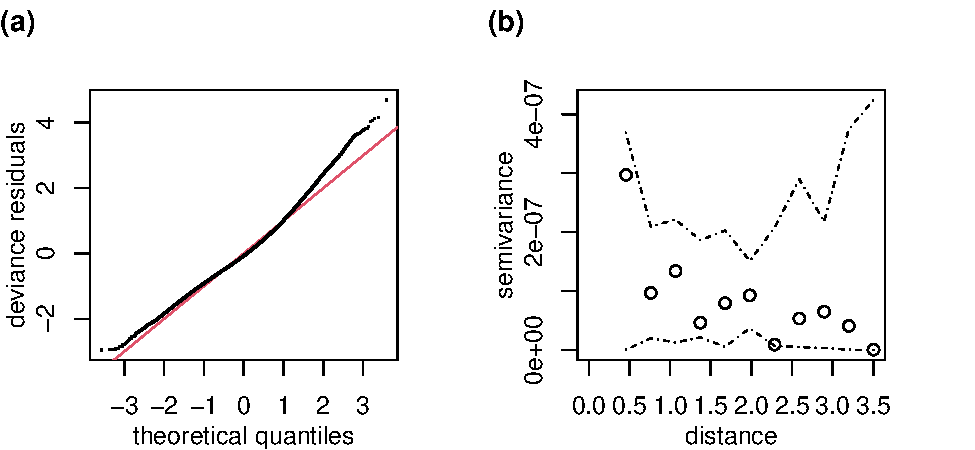
\includegraphics{thesis_files/figure-latex/unnamed-chunk-12-1.pdf}
\caption{\label{fig:unnamed-chunk-12}\label{fig:check} Dialog plot for GAM. Figure (a) is the QQ norm plot of residuals and (b) is the spatial progress semivarigam plot.}
\end{figure}
\hypertarget{prediction-effeciency}{%
\section{Prediction effeciency}\label{prediction-effeciency}}

One concern is whether the covariates effective for prediction. To avoid overfitting, we tested the ability of the covariates to predict flows using 5-fold cross-validation on the complete data set. The R code to carry out the procedure is as Appendix \ref{code}. The values of RMSPE, MAPE, and MdAPE are listed in Table. \ref{tab:MSE}.
\begin{table}[!h]

\caption{\label{tab:unnamed-chunk-13}\label{tab:MSE} RMSPE, MAPE and MdAPE scores when the model excludes covariates and contains covariates}
\centering
\fontsize{10}{12}\selectfont
\begin{tabular}[t]{lrr}
\toprule
Error criteria & Model without covariates & Model with covariates\\
\midrule
RMSPE & 2.99 & 1.61\\
MAPE & 2.33 & 1.25\\
MdAPE & 1.86 & 0.99\\
\bottomrule
\end{tabular}
\end{table}
The mean RMSPE, MAPE and MdAPE values for model cross-validation are smaller when the model includes covariates Catchment Area and Maximum Altitude (1.61, 1.25 and 0.99, respectively) than when the model does not include covariates (2.99, 2.33 and 1.86, respectively). The five-folder cross validation indicates that it is more effective in predicting to include the covariates in the model under the three criteria.

\hypertarget{scottish-hydrological-features}{%
\section{Scottish hydrological features}\label{scottish-hydrological-features}}

We apply the model into the full dataset to explore how the average daily flows in Scotland vary over time and space. To balance the computational cost and accuracy, we choose the k values as follows. For the univariate terms, temporal and seasonal effects, the B-splines are proposed. The k of temporal effect function, say, \(s_1(t),\;t=\) year(1989-2015), is selected as 6 and the k of seasonal effect, \(s_2(d)\), \(d=\) the day of the year (1-365), is choose as 6. The smooth functions of bivariate terms and interaction terms are cubic regression splines. We make k equals to 49 in the bivariate term \(s_3(z)\), \(z=\)(Longitude, Latitude), which represents the spatial effect. The k values of interaction items \(s_4(t,d)\), \(s_5(t,z)\), and \(s_6(d,z)\) are setted as upper limit on the degree of freedom in the smooth functions.

The DER of the full model is 71\%, which fits and explains the data with 640575 observations well. All covariates and items are significant at 0.05 with p values less than 0.0001. The estimated coefficients of Catchment Area and Max Altitude are 0.0001 and 0.0016 respectively. They have a positive relationship with Flow. Catchments with high Max Altitude and large areas usually contain mountains. The streams go down from the peaks, which leads to a large flow. It keeps constant with the exploratory analysis.

Fig.\ref{fig:what} shows the main effects of temporal, seasonal, and spatial smooth items respectively. Fig.\ref{fig:what}(a) draws the variation of streamflow in a year. The flow in Scotland has maintained obvious seasonal characteristics. The minimum flow is reached on about the 200th day, that is, July 19. It is small in summer and more in winter. This is related to the heavy snowfall in winter. According to Fig.\ref{fig:what}(b), the temporal trend shows an overall rise, which may be affected by glacier melting. Werritty \& Sugden (2012) also mentioned this in the impact of global warming on the climate in Scotland.

Fig.\ref{fig:what}(c) reveals the spatial features of the discharge. In high-altitude mountains, the flow is often small. The river originates from here and flows downward, producing a large flow in the surrounding area. In the Highland area of North-western Scotland, the color is darker where mountains are located, for example, on the Grampian Mountains. After water flows down from high latitudes, it reaches its maximum in the rift valley in the Central Lowland. Mountains in the Southern Uplands block the streamflow. The water originated here also flows to the low-lying central rift valley, which together with the water flow in the North leads to a large flow in the central region, while the Southern Uplands have the lowest flow.
\begin{figure}
\centering
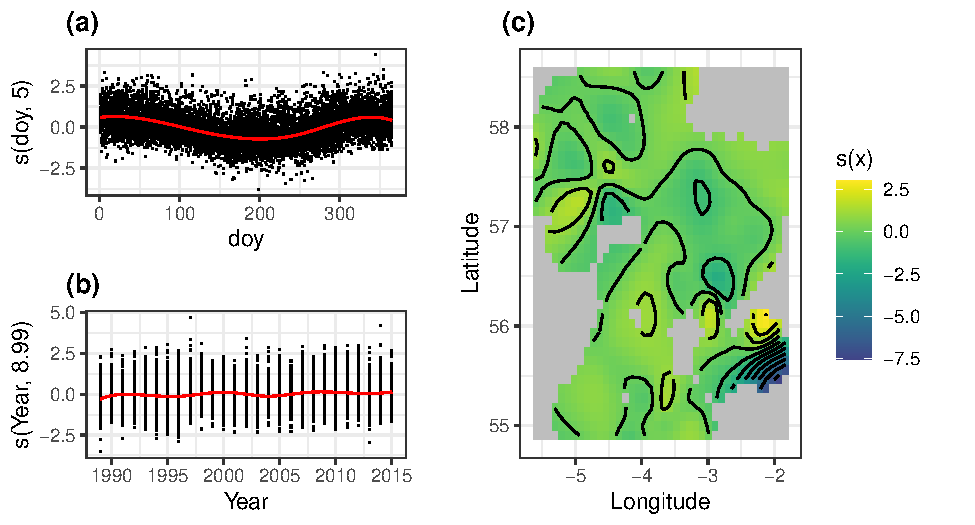
\includegraphics{thesis_files/figure-latex/unnamed-chunk-15-1.pdf}
\caption{\label{fig:unnamed-chunk-15}\label{fig:what} Estimated (a)temporal, (b)seasonal and (c)spatial smooth items.}
\end{figure}
Fig.\ref{fig:sha} exhibits the estimated interactions of temporal-seasonal, temporal-spatial, and seasonal-spatial smooth items. Fig.\ref{fig:sha}(a) depicts that as the year moves, the minimum values of the interaction of doy with year move from summer to winter and the maximum values roll from spring to autumn. Fig.\ref{fig:sha}(b) graphs the spatial distribution of flows in the different seasons, using the 1st, 92th, 182th, and 274th days of the year (i.e.~1 January, 1 April, 1 July, and 1 October) as facets. In winter (doy=1), flows are small in the Highlands with mountains and large in the Central Lowlands. Little variation in flows across the territory is more equitable in spring (doy=92). Summer (doy=182) is the opposite of winter, with high flows in the mountains and low flows in the lowlands. In autumn (doy=274), the tall mountains in the west obstruct the flow of air from the Atlantic Ocean and consequently the flow is high while low on the east coast. Fig.\ref{fig:sha}(c) traces the spatial distribution of flows across years from 1990 to 2015 at 5-year intervals. In particular, the effect of the Atlantic Current was especially pronounced in 1990, with high flows on the west coast and low flows on the east coast. The influence of elevation on flows was dominant in 2015, with high flows in high terrain and low flows in lowland areas. The rest of the years were more evenly distributed spatially, but with a rising trend overall.
\begin{figure}
\centering
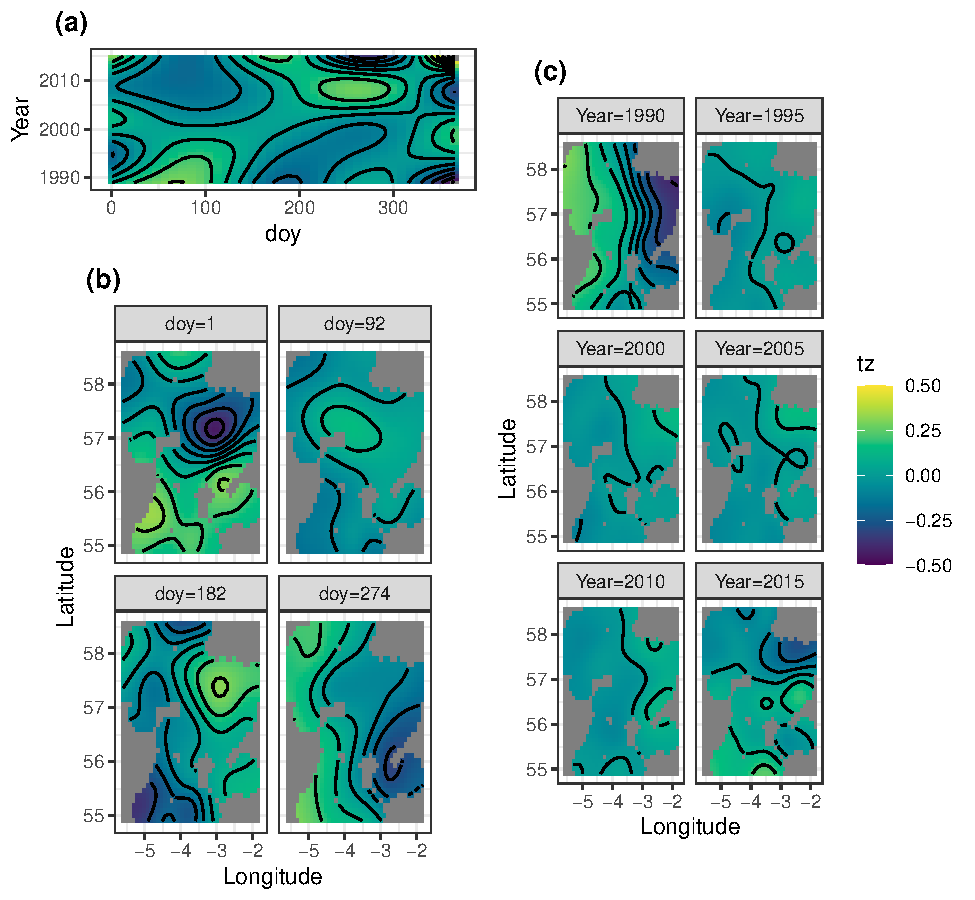
\includegraphics{thesis_files/figure-latex/unnamed-chunk-16-1.pdf}
\caption{\label{fig:unnamed-chunk-16}\label{fig:sha} Estimated interactions of (a)temporal-seasonal, (b)temporal-spatial and (c)seasonal-spatial smooth items.}
\end{figure}
We employed the GAM model combined with AR(1) model to forecast flows in Scotland from 2021 to 2030. Table. \ref{tab:pre} lists the predictions of average flow in Scotland over the four seasons at 3-year intervals for different years. The forecasts demonstrate a progressive increase in average flows for each season. Winter has the heaviest flows, while the lowest flows are pushed from summer to autumn.
\begin{table}[!h]

\caption{\label{tab:unnamed-chunk-17}\label{tab:pre} Preditions of average flow in Scotand from 2021 to 2030 by 3 years over the four seasons}
\centering
\fontsize{10}{12}\selectfont
\begin{tabular}[t]{rrrrr}
\toprule
Year & Winter & Spring & Summer & Autumn\\
\midrule
2021 & 3.59 & 2.55 & 1.97 & 1.40\\
2024 & 4.07 & 2.92 & 2.27 & 1.35\\
2027 & 4.55 & 3.29 & 2.57 & 1.29\\
2030 & 5.04 & 3.66 & 2.87 & 1.23\\
\bottomrule
\end{tabular}
\end{table}
\hypertarget{conclusions}{%
\section{Conclusions}\label{conclusions}}

The previous analysis provides answers to the three questions posed in Chapter 1. Flows in Scotland are progressively increasing and swing on a five-year periodicity. Within each year, winter flows are high and summer flows are low. Yet the difference is diminishing, with flows intensifying in summer and reducing in winter. In terms of spatial distribution, flows are relatively low in Highlands and high in the Central Lowland. Flows are also in excess of the East Coast on the West Coast. Further, we found the spatio-temporal characteristics of Scottish flows. The west coast was distinctly higher than the east coast in the early 1990s, with the rest of the years mainly following the low latitude, high flow characteristics, which were reinforced in the late decade at low latitudes. During the year, winter-summer flows are mainly determined by latitude, with autumn influenced by Atlantic currents. At last, the covariates catchment area and maximum latitude noticeably enhance the ability of models to predict flows in Scotland. Scottish average flows are forecast to continue to rise between 2021 and 2030.

\hypertarget{conclusion}{%
\chapter{Conclusions and discussions}\label{conclusion}}

\hypertarget{summary-of-conclusions}{%
\section{Summary of conclusions}\label{summary-of-conclusions}}

We assembles 640,575 flow observations from 65 gauging stations in Scotland over 27 years from 1989 to 2015, and the dependent variables of Gaussian distribution, Gaussian distribution log link function, Gamma distribution log link function, and log-transformed Gaussian distribution with catchment area and maximum latitude as covariates are modelled respectively, for time effect, seasonal effect, spatial effect, and interactions via GAMs. We select and check the candidate models to analyse the hydrological characteristics of Scotland. There is an upward trend in Scottish flows over time, with a seasonal feature of small summer flows and large winter flows, and the disparity is narrowing. Spatially, it adheres to two patterns, the higher the latitude the lower the flow and the greater the flow on the west coast than on the east coast, the latter of which is strengthened in recent years. The area and the maximum latitude of the catchment enable distinctly more accurate predictions. The study concludes by forecasting an upward trend in average flows in Scotland from 2021 to 2030.

The approach in this paper is computationally fast and substantially reduces the time required to fit the model by choosing appropriate algorithms and parameters. The results are robust by selecting models and testing their effectiveness through a variety of criteria. Compared to machine learning methods which are regarded as black-box, the interpretation and visualization are stronger. The issue of over-fitting is partly reduced by penalty terms and cross-validation. This paper fills a gap in Scottish flow studies by analysing the hydrological characteristics of entire Scotland.

\hypertarget{discussion-of-limitations}{%
\section{Discussion of limitations}\label{discussion-of-limitations}}

A number of limitations need to be noted regarding the present study. First, uncertainty, essential in hydrological forecasting, is not adequately estimated, which may lead to inaccurate outcomes. Second, not all possible covariates are considered in the GAM, for example, precipitation is a potential predictor variable and this variable is not included in this study due to the limitations of data availability. Third, We do not compare the properties of GAMs with other popular methods due to computational speed constraints.

\hypertarget{further-analysis}{%
\section{Further analysis}\label{further-analysis}}

Given the limitations of the methodology in this paper, future work may include the following. First, another possible area of future research would be to investigate the uncertainty of streamflow trends.
Bootstrap is suggested to evaluate the uncertainty. Secondly, the performance of the model could potentially be boosted by trying out more covariates and various models, for example, spatio-temporal models with the integrated nested Laplace approximation approach.

\appendix

\hypertarget{infor}{%
\chapter{Information of 13 selected gauging stations}\label{infor}}

Table \ref{tab:information} is a summary of selected gauging stations. The distributions of sample data are similar to the complete data.
\begin{table}[!h]

\caption{\label{tab:unnamed-chunk-18}\label{tab:information} Information for 13 gauging stations for model selection .}
\centering
\fontsize{10}{12}\selectfont
\begin{tabular}[t]{lrrrrr}
\toprule
Station & Longitude & Latitude & \makecell[c]{Catchment\\area} & \makecell[c]{Max\\altitude} & \makecell[c]{Mean\\flow}\\
\midrule
Allt Deveron at Cabrach & -3.04 & 57.35 & 67.0 & 720.8 & 1.62\\
Almond at Almondbank & -3.51 & 56.42 & 174.8 & 926.2 & 5.74\\
Clyde at Hazelbank & -3.85 & 55.69 & 1092.9 & 745.2 & 32.70\\
Conon at Moy Bridge & -4.54 & 57.56 & 961.8 & 1103.4 & 56.01\\
Dulnain at Balnaan Bridge & -3.70 & 57.30 & 272.2 & 875.4 & 6.35\\
\addlinespace
Gairn at Invergairn & -3.07 & 57.06 & 150.0 & 1160.4 & 3.77\\
Irvine at Glenfield & -4.50 & 55.60 & 218.0 & 383.3 & 6.13\\
Scar Water at Capenoch & -3.82 & 55.23 & 142.0 & 597.2 & 6.25\\
Stinchar at Balnowlart & -4.97 & 55.11 & 341.0 & 623.8 & 10.93\\
Strathy at Strathy Bridge & -4.00 & 58.56 & 111.8 & 345.1 & 2.66\\
\addlinespace
Tummel at Pitlochry & -3.72 & 56.70 & 1670.0 & 1133.4 & 77.70\\
Tweed at Norham & -2.16 & 55.72 & 4390.0 & 838.0 & 85.67\\
Ugie at Inverugie & -1.83 & 57.53 & 325.0 & 233.7 & 5.02\\
\bottomrule
\end{tabular}
\end{table}
\hypertarget{code}{%
\chapter{Code for cross validates method}\label{code}}

The cross validates method was carried out by the following code with three functions, LOOCV1, LOOCV2, and ACC.
\begin{Shaded}
\begin{Highlighting}[]
\CommentTok{\# We first split the complete data set randomly.}
\CommentTok{\# The objective data is the full dataset.}
\CommentTok{\# There are 65 gauging stations.}
\NormalTok{ x }\OtherTok{\textless{}{-}} \FunctionTok{unique}\NormalTok{(data}\SpecialCharTok{$}\NormalTok{ID)}
\NormalTok{ y }\OtherTok{\textless{}{-}} \FunctionTok{as.data.frame}\NormalTok{(}\FunctionTok{matrix}\NormalTok{(}\ConstantTok{NA}\NormalTok{, }\AttributeTok{ncol =} \DecValTok{2}\NormalTok{, }\AttributeTok{nrow =} \DecValTok{65}\NormalTok{))}
 \FunctionTok{names}\NormalTok{(y) }\OtherTok{\textless{}{-}} \FunctionTok{c}\NormalTok{(}\StringTok{"ID"}\NormalTok{,}\StringTok{"index"}\NormalTok{)}
\CommentTok{\# We create five indexes for the five subset}
 \ControlFlowTok{for}\NormalTok{ (i }\ControlFlowTok{in} \DecValTok{1}\SpecialCharTok{:}\DecValTok{5}\NormalTok{)\{}
\NormalTok{   x1 }\OtherTok{\textless{}{-}} \FunctionTok{sample}\NormalTok{(x, }\DecValTok{13}\NormalTok{)}
\NormalTok{   x }\OtherTok{\textless{}{-}}\NormalTok{ x[}\SpecialCharTok{{-}}\FunctionTok{which}\NormalTok{(x }\SpecialCharTok{\%in\%}\NormalTok{ x1)]}
\NormalTok{   x1 }\OtherTok{\textless{}{-}} \FunctionTok{data.frame}\NormalTok{(}\AttributeTok{ID =}\NormalTok{ x1, }\AttributeTok{index =}\NormalTok{ i)}
\NormalTok{   y[(}\DecValTok{13}\SpecialCharTok{*}\NormalTok{(i}\DecValTok{{-}1}\NormalTok{)}\SpecialCharTok{+}\DecValTok{1}\NormalTok{)}\SpecialCharTok{:}\NormalTok{(}\DecValTok{13}\SpecialCharTok{*}\NormalTok{i),] }\OtherTok{\textless{}{-}}\NormalTok{ x1}
\NormalTok{ \}}
 
\CommentTok{\# RMSPE, MAPE and MdAPE values for model without covariates}
\NormalTok{LOOCV1 }\OtherTok{\textless{}{-}} \ControlFlowTok{function}\NormalTok{(x)\{}
\NormalTok{  subdata }\OtherTok{\textless{}{-}}\NormalTok{ data }\SpecialCharTok{\%\textgreater{}\%} \FunctionTok{filter}\NormalTok{(index }\SpecialCharTok{!=}\NormalTok{ x)}
\NormalTok{  subdata2 }\OtherTok{\textless{}{-}}\NormalTok{ data }\SpecialCharTok{\%\textgreater{}\%} \FunctionTok{filter}\NormalTok{(index }\SpecialCharTok{==}\NormalTok{ x)}
\NormalTok{  fit }\OtherTok{\textless{}{-}} \FunctionTok{bam}\NormalTok{(}\FunctionTok{log}\NormalTok{(Flow) }\SpecialCharTok{\textasciitilde{}} 
               \FunctionTok{s}\NormalTok{(doy, }\AttributeTok{bs =} \StringTok{"bs"}\NormalTok{, }\AttributeTok{m =} \FunctionTok{c}\NormalTok{(}\DecValTok{3}\NormalTok{,}\DecValTok{2}\NormalTok{), }\AttributeTok{k =} \DecValTok{6}\NormalTok{) }\SpecialCharTok{+} 
               \FunctionTok{s}\NormalTok{(Year, }\AttributeTok{bs =} \StringTok{"bs"}\NormalTok{, }\AttributeTok{m =} \FunctionTok{c}\NormalTok{(}\DecValTok{3}\NormalTok{,}\DecValTok{2}\NormalTok{), }\AttributeTok{k =} \DecValTok{6}\NormalTok{) }\SpecialCharTok{+}     
               \FunctionTok{te}\NormalTok{(Longitude, Latitude, }
                  \AttributeTok{bs =} \StringTok{"cr"}\NormalTok{, }\AttributeTok{k =} \DecValTok{13}\NormalTok{) }\SpecialCharTok{+}
               \FunctionTok{ti}\NormalTok{(doy, Year, }
                  \AttributeTok{bs =} \StringTok{"cr"}\NormalTok{, }\AttributeTok{k =} \DecValTok{6}\NormalTok{)}\SpecialCharTok{+}
               \FunctionTok{ti}\NormalTok{(Longitude, Latitude, doy, }\AttributeTok{d=}\FunctionTok{c}\NormalTok{(}\DecValTok{2}\NormalTok{,}\DecValTok{1}\NormalTok{), }
                  \AttributeTok{bs =} \StringTok{"cr"}\NormalTok{, }\AttributeTok{k =} \DecValTok{6}\NormalTok{) }\SpecialCharTok{+}
               \FunctionTok{ti}\NormalTok{(Longitude, Latitude, Year, }\AttributeTok{d=}\FunctionTok{c}\NormalTok{(}\DecValTok{2}\NormalTok{,}\DecValTok{1}\NormalTok{), }
                  \AttributeTok{bs =} \StringTok{"cr"}\NormalTok{, }\AttributeTok{k =} \DecValTok{6}\NormalTok{), }
             \AttributeTok{method =} \StringTok{"fREML"}\NormalTok{,}
             \AttributeTok{data =}\NormalTok{ subdata)}
\NormalTok{  pred }\OtherTok{\textless{}{-}} \FunctionTok{predict}\NormalTok{(fit, subdata2)}
\NormalTok{  res }\OtherTok{\textless{}{-}} \FunctionTok{log}\NormalTok{(subdata2}\SpecialCharTok{$}\NormalTok{Flow) }\SpecialCharTok{{-}}\NormalTok{ pred}
\NormalTok{  RMSPE }\OtherTok{\textless{}{-}} \FunctionTok{sqrt}\NormalTok{(}\FunctionTok{mean}\NormalTok{(res}\SpecialCharTok{\^{}}\DecValTok{2}\NormalTok{))}
\NormalTok{  MAPE }\OtherTok{\textless{}{-}} \FunctionTok{mean}\NormalTok{(}\FunctionTok{abs}\NormalTok{(res))}
\NormalTok{  MdAPE }\OtherTok{\textless{}{-}} \FunctionTok{median}\NormalTok{(}\FunctionTok{abs}\NormalTok{(res))}
\NormalTok{  ACC }\OtherTok{\textless{}{-}} \FunctionTok{c}\NormalTok{(RMSPE, MAPE,MdAPE)}
  \FunctionTok{return}\NormalTok{(ACC)}
\NormalTok{\}}

\CommentTok{\# RMSPE, MAPE and MdAPE values for model without covariates}
\NormalTok{LOOCV2 }\OtherTok{\textless{}{-}} \ControlFlowTok{function}\NormalTok{(x)\{}
\NormalTok{  subdata }\OtherTok{\textless{}{-}}\NormalTok{ data }\SpecialCharTok{\%\textgreater{}\%} \FunctionTok{filter}\NormalTok{(index }\SpecialCharTok{!=}\NormalTok{ x)}
\NormalTok{  subdata2 }\OtherTok{\textless{}{-}}\NormalTok{ data }\SpecialCharTok{\%\textgreater{}\%} \FunctionTok{filter}\NormalTok{(index }\SpecialCharTok{==}\NormalTok{ x)}
\NormalTok{  fit }\OtherTok{\textless{}{-}} \FunctionTok{bam}\NormalTok{(}\FunctionTok{log}\NormalTok{(Flow) }\SpecialCharTok{\textasciitilde{}}\NormalTok{ Catchment.Area }\SpecialCharTok{+}\NormalTok{ Max.Altitude }\SpecialCharTok{+}
                 \FunctionTok{s}\NormalTok{(doy, }\AttributeTok{bs =} \StringTok{"bs"}\NormalTok{, }\AttributeTok{m =} \FunctionTok{c}\NormalTok{(}\DecValTok{3}\NormalTok{,}\DecValTok{2}\NormalTok{), }\AttributeTok{k =} \DecValTok{6}\NormalTok{) }\SpecialCharTok{+} 
                 \FunctionTok{s}\NormalTok{(Year, }\AttributeTok{bs =} \StringTok{"bs"}\NormalTok{, }\AttributeTok{m =} \FunctionTok{c}\NormalTok{(}\DecValTok{3}\NormalTok{,}\DecValTok{2}\NormalTok{), }\AttributeTok{k =} \DecValTok{6}\NormalTok{) }\SpecialCharTok{+} 
                 \FunctionTok{te}\NormalTok{(Longitude, Latitude, }
                    \AttributeTok{bs =} \StringTok{"cr"}\NormalTok{, }\AttributeTok{k =} \DecValTok{13}\NormalTok{) }\SpecialCharTok{+}
                 \FunctionTok{ti}\NormalTok{(doy, Year, }
                    \AttributeTok{bs =} \StringTok{"cr"}\NormalTok{, }\AttributeTok{k =} \DecValTok{6}\NormalTok{)}\SpecialCharTok{+}
                 \FunctionTok{ti}\NormalTok{(Longitude, Latitude, doy, }\AttributeTok{d=}\FunctionTok{c}\NormalTok{(}\DecValTok{2}\NormalTok{,}\DecValTok{1}\NormalTok{), }
                    \AttributeTok{bs =} \StringTok{"cr"}\NormalTok{, }\AttributeTok{k =} \DecValTok{6}\NormalTok{) }\SpecialCharTok{+}
                 \FunctionTok{ti}\NormalTok{(Longitude, Latitude, Year, }\AttributeTok{d=}\FunctionTok{c}\NormalTok{(}\DecValTok{2}\NormalTok{,}\DecValTok{1}\NormalTok{), }
                    \AttributeTok{bs =} \StringTok{"cr"}\NormalTok{, }\AttributeTok{k =} \DecValTok{6}\NormalTok{), }
               \AttributeTok{method =} \StringTok{"fREML"}\NormalTok{,}
               \AttributeTok{data =}\NormalTok{ subdata)}
\NormalTok{  pred }\OtherTok{\textless{}{-}} \FunctionTok{predict}\NormalTok{(fit, subdata2)}
\NormalTok{  res }\OtherTok{\textless{}{-}} \FunctionTok{log}\NormalTok{(subdata2}\SpecialCharTok{$}\NormalTok{Flow) }\SpecialCharTok{{-}}\NormalTok{ pred}
\NormalTok{  RMSPE }\OtherTok{\textless{}{-}} \FunctionTok{sqrt}\NormalTok{(}\FunctionTok{mean}\NormalTok{(res}\SpecialCharTok{\^{}}\DecValTok{2}\NormalTok{))}
\NormalTok{  MAPE }\OtherTok{\textless{}{-}} \FunctionTok{mean}\NormalTok{(}\FunctionTok{abs}\NormalTok{(res))}
\NormalTok{  MdAPE }\OtherTok{\textless{}{-}} \FunctionTok{median}\NormalTok{(}\FunctionTok{abs}\NormalTok{(res))}
\NormalTok{  ACC }\OtherTok{\textless{}{-}} \FunctionTok{c}\NormalTok{(RMSPE, MAPE,MdAPE)}
  \FunctionTok{return}\NormalTok{(ACC)}
\NormalTok{\}}

\CommentTok{\# Let each of the five subsets be a test set}
\NormalTok{ACC1 }\OtherTok{\textless{}{-}} \FunctionTok{list}\NormalTok{(}\FunctionTok{LOOCV1}\NormalTok{(}\DecValTok{1}\NormalTok{), }\FunctionTok{LOOCV1}\NormalTok{(}\DecValTok{2}\NormalTok{), }\FunctionTok{LOOCV1}\NormalTok{(}\DecValTok{3}\NormalTok{), }\FunctionTok{LOOCV1}\NormalTok{(}\DecValTok{4}\NormalTok{), }\FunctionTok{LOOCV1}\NormalTok{(}\DecValTok{5}\NormalTok{))}
\NormalTok{ACC2 }\OtherTok{\textless{}{-}} \FunctionTok{list}\NormalTok{(}\FunctionTok{LOOCV2}\NormalTok{(}\DecValTok{1}\NormalTok{), }\FunctionTok{LOOCV2}\NormalTok{(}\DecValTok{2}\NormalTok{), }\FunctionTok{LOOCV2}\NormalTok{(}\DecValTok{3}\NormalTok{), }\FunctionTok{LOOCV2}\NormalTok{(}\DecValTok{4}\NormalTok{), }\FunctionTok{LOOCV2}\NormalTok{(}\DecValTok{5}\NormalTok{))}

\CommentTok{\# Calculate the mean values of five test set}
\NormalTok{acc }\OtherTok{\textless{}{-}} \ControlFlowTok{function}\NormalTok{(x)\{}
\NormalTok{  RMSPE }\OtherTok{\textless{}{-}} \FunctionTok{numeric}\NormalTok{()}
\NormalTok{  MAPE }\OtherTok{\textless{}{-}} \FunctionTok{numeric}\NormalTok{()}
\NormalTok{  MdAPE }\OtherTok{\textless{}{-}} \FunctionTok{numeric}\NormalTok{()}
  \ControlFlowTok{for}\NormalTok{ (i }\ControlFlowTok{in} \DecValTok{1}\SpecialCharTok{:}\DecValTok{5}\NormalTok{)\{}
\NormalTok{    RMSPE[i] }\OtherTok{\textless{}{-}}\NormalTok{  x[[i]][}\DecValTok{1}\NormalTok{]}
\NormalTok{    MAPE[i] }\OtherTok{\textless{}{-}}\NormalTok{ x[[i]][}\DecValTok{2}\NormalTok{]}
\NormalTok{    MdAPE[i] }\OtherTok{\textless{}{-}}\NormalTok{ x[[i]][}\DecValTok{3}\NormalTok{]}
\NormalTok{  \}}
\NormalTok{  acc }\OtherTok{\textless{}{-}} \FunctionTok{c}\NormalTok{(}\FunctionTok{mean}\NormalTok{(RMSPE), }\FunctionTok{mean}\NormalTok{(MAPE),}\FunctionTok{mean}\NormalTok{(MdAPE))}
  \FunctionTok{return}\NormalTok{(acc)}
\NormalTok{\}}

\FunctionTok{acc}\NormalTok{(ACC1)}
\FunctionTok{acc}\NormalTok{(ACC2)}
\end{Highlighting}
\end{Shaded}
\backmatter

\hypertarget{references}{%
\chapter*{References}\label{references}}
\addcontentsline{toc}{chapter}{References}

\markboth{References}{References}

\noindent

\setlength{\parindent}{-0.20in}

\hypertarget{refs}{}
\begin{CSLReferences}{1}{0}
\leavevmode\hypertarget{ref-akaike1998}{}%
Akaike, H. (1998). Information theory and an extension of the maximum likelihood principle (pp. 199--213). Springer New York. http://doi.org/\href{https://doi.org/10.1007/978-1-4612-1694-0_15}{10.1007/978-1-4612-1694-0\_15}

\leavevmode\hypertarget{ref-black1995}{}%
Black, A. R. (1995). Major flooding and increased flood frequency in Scotland since 1988. \emph{Physics and Chemistry of the Earth}, \emph{20}(5-6), 463--468. http://doi.org/\href{https://doi.org/10.1016/s0079-1946(96)00007-9}{10.1016/s0079-1946(96)00007-9}

\leavevmode\hypertarget{ref-black1997}{}%
Black, Andrew R., \& Werritty, A. (1997). Seasonality of flooding: a case study of North Britain. \emph{Journal of Hydrology}, \emph{195}(1-4), 1--25. http://doi.org/\href{https://doi.org/10.1016/s0022-1694(96)03264-7}{10.1016/s0022-1694(96)03264-7}

\leavevmode\hypertarget{ref-bobee1993}{}%
Bobee, B., Perreault, L., \& Ashkar, F. (1993). Two kinds of moment ratio diagrams and their applications in hydrology. \emph{Stochastic Hydrology and Hydraulics}, \emph{7}(1), 41--65. http://doi.org/\href{https://doi.org/10.1007/bf01581566}{10.1007/bf01581566}

\leavevmode\hypertarget{ref-buckland1997}{}%
Buckland, S. T., Burnham, K. P., \& Augustin, N. H. (1997). Model selection: An integral part of inference. \emph{Biometrics}, \emph{53}(2), 603. http://doi.org/\href{https://doi.org/10.2307/2533961}{10.2307/2533961}

\leavevmode\hypertarget{ref-franco-villoria2018}{}%
Franco-Villoria, M., Scott, M., \& Hoey, T. (2018). Spatiotemporal modeling of hydrological return levels: A quantile regression approach. \emph{Environmetrics}, \emph{30}(2), e2522. http://doi.org/\href{https://doi.org/10.1002/env.2522}{10.1002/env.2522}

\leavevmode\hypertarget{ref-griffiths2006}{}%
Griffiths, J., Binley, A., Crook, N., Nutter, J., Young, A., \& Fletcher, S. (2006). Streamflow generation in the Pang and Lambourn catchments, Berkshire, UK. \emph{Journal of Hydrology}, \emph{330}(1-2), 71--83. http://doi.org/\href{https://doi.org/10.1016/j.jhydrol.2006.04.044}{10.1016/j.jhydrol.2006.04.044}

\leavevmode\hypertarget{ref-harrigan2018}{}%
Harrigan, S., Prudhomme, C., Parry, S., Smith, K., \& Tanguy, M. (2018). Benchmarking ensemble streamflow prediction skill in the UK. \emph{Hydrology and Earth System Sciences}, \emph{22}(3), 2023--2039. http://doi.org/\href{https://doi.org/10.5194/hess-22-2023-2018}{10.5194/hess-22-2023-2018}

\leavevmode\hypertarget{ref-iorgulescu2004}{}%
Iorgulescu, I., \& Beven, K. J. (2004). Nonparametric direct mapping of rainfall-runoff relationships: An alternative approach to data analysis and modeling? \emph{Water Resources Research}, \emph{40}(8). http://doi.org/\href{https://doi.org/10.1029/2004wr003094}{10.1029/2004wr003094}

\leavevmode\hypertarget{ref-kisi2011}{}%
Kisi, O., \& Cimen, M. (2011). A wavelet-support vector machine conjunction model for monthly streamflow forecasting. \emph{Journal of Hydrology}, \emph{399}(1-2), 132--140. http://doi.org/\href{https://doi.org/10.1016/j.jhydrol.2010.12.041}{10.1016/j.jhydrol.2010.12.041}

\leavevmode\hypertarget{ref-10.5285ux2f10d419c8-8f65-4b85-a78a-3d6e0485fa1f}{}%
Kral, M. ;Dixon., F.;Fry. (2015). Integrated hydrological units of the united kingdom: catchments. NERC Environmental Information Data Centre. http://doi.org/\href{https://doi.org/10.5285/10d419c8-8f65-4b85-a78a-3d6e0485fa1f}{10.5285/10d419c8-8f65-4b85-a78a-3d6e0485fa1f}

\leavevmode\hypertarget{ref-li2019}{}%
Li, Z., \& Wood, S. N. (2019). Faster model matrix crossproducts for large generalized linear models with discretized covariates. \emph{Statistics and Computing}, \emph{30}(1), 19--25. http://doi.org/\href{https://doi.org/10.1007/s11222-019-09864-2}{10.1007/s11222-019-09864-2}

\leavevmode\hypertarget{ref-naveau2020}{}%
Naveau, P., Hannart, A., \& Ribes, A. (2020). Statistical Methods for Extreme Event Attribution in Climate Science. \emph{Annual Review of Statistics and Its Application}, \emph{7}(1), 89--110. http://doi.org/\href{https://doi.org/10.1146/annurev-statistics-031219-041314}{10.1146/annurev-statistics-031219-041314}

\leavevmode\hypertarget{ref-prosdocimi2014}{}%
Prosdocimi, I., Kjeldsen, T. R., \& Svensson, C. (2014). Non-stationarity in annual and seasonal series of peak flow and precipitation in the UK. \emph{Natural Hazards and Earth System Sciences}, \emph{14}(5), 1125--1144. http://doi.org/\href{https://doi.org/10.5194/nhess-14-1125-2014}{10.5194/nhess-14-1125-2014}

\leavevmode\hypertarget{ref-scheipl2008}{}%
Scheipl, F., Greven, S., \& Küchenhoff, H. (2008). Size and power of tests for a zero random effect variance or polynomial regression in additive and linear mixed models. \emph{Computational Statistics \& Data Analysis}, \emph{52}(7), 3283--3299. http://doi.org/\href{https://doi.org/10.1016/j.csda.2007.10.022}{10.1016/j.csda.2007.10.022}

\leavevmode\hypertarget{ref-Maxim2013}{}%
Shcherbakov, M., Brebels, A., Shcherbakova, N. L., Tyukov, A., Janovsky, T. A., \& Kamaev, V. A. (2013). A survey of forecast error measures. \emph{World Applied Sciences Journal}, \emph{24}, 171--176. http://doi.org/\href{https://doi.org/10.5829/idosi.wasj.2013.24.itmies.80032}{10.5829/idosi.wasj.2013.24.itmies.80032}

\leavevmode\hypertarget{ref-shortridge2016}{}%
Shortridge, J. E., Guikema, S. D., \& Zaitchik, B. F. (2016). Machine learning methods for empirical streamflow simulation: a comparison of model accuracy, interpretability, and uncertainty in seasonal watersheds. \emph{Hydrology and Earth System Sciences}, \emph{20}(7), 2611--2628. http://doi.org/\href{https://doi.org/10.5194/hess-20-2611-2016}{10.5194/hess-20-2611-2016}

\leavevmode\hypertarget{ref-smith1994}{}%
Smith, K., \& Bennett, A. M. (1994). Recently increased river discharge in Scotland: effects on flow hydrology and some implications for water management. \emph{Applied Geography}, \emph{14}(2), 123--133. http://doi.org/\href{https://doi.org/10.1016/0143-6228(94)90056-6}{10.1016/0143-6228(94)90056-6}

\leavevmode\hypertarget{ref-solomatine2008}{}%
Solomatine, D. P., \& Ostfeld, A. (2008). Data-driven modelling: some past experiences and new approaches. \emph{Journal of Hydroinformatics}, \emph{10}(1), 3--22. http://doi.org/\href{https://doi.org/10.2166/hydro.2008.015}{10.2166/hydro.2008.015}

\leavevmode\hypertarget{ref-soulsby2002}{}%
Soulsby, C., Black, A. R., \& Werritty, A. (2002). Hydrology in Scotland: towards a scientific basis for the sustainable management of freshwater resources{{}}foreword to thematic issue. \emph{Science of The Total Environment}, \emph{294}(1-3), 3--11. http://doi.org/\href{https://doi.org/10.1016/s0048-9697(02)00048-7}{10.1016/s0048-9697(02)00048-7}

\leavevmode\hypertarget{ref-werritty2012}{}%
Werritty, A., \& Sugden, D. (2012). Climate change and Scotland: recent trends and impacts. \emph{Earth and Environmental Science Transactions of the Royal Society of Edinburgh}, \emph{103}(2), 133--147. http://doi.org/\href{https://doi.org/10.1017/s1755691013000030}{10.1017/s1755691013000030}

\leavevmode\hypertarget{ref-wood2014}{}%
Wood, S. N., Goude, Y., \& Shaw, S. (2014). Generalized additive models for large data sets. \emph{Journal of the Royal Statistical Society: Series C (Applied Statistics)}, \emph{64}(1), 139--155. http://doi.org/\href{https://doi.org/10.1111/rssc.12068}{10.1111/rssc.12068}

\leavevmode\hypertarget{ref-wood2017}{}%
Wood, S. N., Li, Z., Shaddick, G., \& Augustin, N. H. (2017). Generalized Additive Models for Gigadata: Modeling the U.K. Black Smoke Network Daily Data. \emph{Journal of the American Statistical Association}, \emph{112}(519), 1199--1210. http://doi.org/\href{https://doi.org/10.1080/01621459.2016.1195744}{10.1080/01621459.2016.1195744}

\leavevmode\hypertarget{ref-yadav2016}{}%
Yadav, S., \& Shukla, S. (2016). Analysis of k-fold cross-validation over hold-out validation on colossal datasets for quality classification. \emph{2016 IEEE 6th International Conference on Advanced Computing (IACC)}. http://doi.org/\href{https://doi.org/10.1109/iacc.2016.25}{10.1109/iacc.2016.25}

\end{CSLReferences}

% Index?

\end{document}
